
\section{Motivation}

As we have just developed a new way to test formality, it would be nice to test it out on some examples. Our gut feeling is that this criteria of having trivial induced product in cohomology is pretty strong. If we are still hoping for results applicable to topological spaces this is especially troubling. Say we have a path-connected topological space $X$---then it has zeroth cohomology $H^0(X;k)\cong k$. If we were to have trivial induced product, we would have $a\cdot [x] = 0$ for any $a\in k$ and $x\in C(X)$, which is only true for $[x]=0$. So this requirement seems to collapse to requiring $H^i(X;k)=0$ for $i>0$, which is really limiting. 

One solution to this is looking at reduced cohomology instead of ``normal'' unreduced cohomology. 

\begin{definition}[Reduced cohomology]
\label{def:reduced_cohomology}
\index{Reduced cohomology}
Let $X$ be a topological space and $C^*(X;k)$ its cochain complex (treated here as an unbounded DG-algebra):
\begin{equation*}
    \cdots \to 0 \to C^0(X)\to C^1(X) \to \cdots \to C^n(X) \to \cdots 
\end{equation*}
We define its augmented cochain DG-algebra, denoted $\widetilde{C}^*(X;k)$ by adding a copy of the ground field $k$ injectively farthest to the left, i.e. 
\begin{equation*}
    \cdots \to 0 \to k \overset{\epsilon}\to C^0(X)\to C^1(X) \to \cdots \to C^n(X) \to \cdots 
\end{equation*}
The cohomology algebra of the augmented cochain complex is called the reduced cohomology algebra of $X$ and is denoted $\widetilde{H}^*(X;k)$.
\end{definition}

If the space $X$ is connected, then $C^0(X;k)\cong k$, meaning that $\widetilde{H}^0(X;k)=0$. This is the important part that will allow us to use the previous results on a topological example, as we have completely removed the problem described above. 

\begin{remark}
This rest of this chapter uses some theory that we will only cover on the absolute surface. This is because the theory is outside the scope, and general vicinity, of this thesis. Thus there are some results we only use, and not prove. References to the results and their proofs are of course provided. 
\end{remark}

\section{Lusternik-Schnirelmann category 1 spaces}

When we do this reduction to reduced cohomology there is a certain class of topological spaces that have exactly the property we desire---that the product in cohomology is trivial. To get to this class we first need to look at a certain homotopy invariant of topological spaces, namely the Lusternik-Schnirelmann category. 

This invariant was originally developed in \cite{lscat} as an invariant on manifolds to be a lower bound for the number of critical points any real valued function on it could have. It has since become a useful---but very difficult to calculate---invariant of topological spaces. 

\begin{definition}[Lusternik-Scnirelmann category]
\label{def:ls_category}
\label{Lusternik-Schnirelmann category}
Let $X$ be a CW complex. The Lusternik-Schnirelmann category of $X$, denoted $\ls(X)$ is the least integer $n$, such that there is a cover of $X$ by $n+1$ subsets $\bigcup_{i=1}^n U_i$ that are contractible in $X$. Being contractible in $X$ means that the inclusion into $X$ is null-homotopic. 
\end{definition}

\begin{example}
\label{ex:suspension}
Let $X$ be a topological space. The \emph{suspension}\index{Suspension of a space} of $X$ is defined to be the topological space
\begin{equation*}
	\Sigma X = X\times I/\sim
\end{equation*}
where $\sim$ is the equivalence relation generated by $(x,1)\sim (y,1)$ and $(x,0)\sim (y,0)$ for all $x,y\in X$. This can be though of as stretching $X$ out into a cylinder, and then collapsing the endpoints into single points. An often used visualization is the following, where we think of $X$ as suspended between the two points---hence the name.
\begin{center}
\def\svgwidth{0.6\textwidth}
\input{images/suspension.pdf_tex}
\end{center}
We see that the suspension is covered by two contractible cones, one above; one below. Hence we get that the Lusternik-Schnirelmann category of any suspension is $1$. 
\end{example}

\begin{example}
Let $X$ be a contractible topological space, then $\ls(X)=0$. This holds in the other direction as well, i.e. if $\ls(X)=0$, then $X$ is contractible.
\end{example}

Recall that \emph{the cup length}\index{Cup length} of a topological space $X$ is the largest integer $n$ such that a chain $[x_1]\cup \cdots \cup [x_n]$ of cohomology classes with $deg|x_i|\geq 1$ is non-zero. We have the following fundamental relation between the cup length and the Lusternik-Schnirelmann category of $X$. The proof is referred to \cite{lscategorybook}.

\begin{lemma}
\label{lem:cup-length_lower_bound}
Let $X$ be a topological space. Then the cup length of $X$ is a lower bound for its Lusternik-Schnirelmann category. 
\end{lemma}

This means that a topological space $X$ such that $\ls(X)=1$ has our desired property that the cup product in the reduced cohomology ring of $X$ is trivial. This is because the cup length has to be equal or lower than the Lusternik-Schnirelmann category, i.e. less than or equal to $1$. By Kadeishvili's theorem\index{Kadeishvili's theorem} (\cref{thm:Kadeishvilis_theorem2}) we get an $\A$-structure $\{m_i\}$ on $H^*(X)$ where $m_1 =0$. As the operation $m_2$ in the $\A$-structure is induced by the cup product we also have $m_2=0$. Hence we know by \ref{thm:cuptrivial_no_massey_then_formal} that the Massey products are the \emph{only} obstructions to formality. But, due to the following result by Rudyak in \cite[Lemma 4.6]{Rudyak}, there are actually none of these obstructions. 

\begin{theorem}
\label{thm:ls1_then_no_massey}
Let $X$ be a CW complex with $\ls(X)\leq 1$ and let the Massey $n$-product\index{Massey product} $\langle x_1, \ldots, x_n\rangle$ be defined with $x_i \in \widetilde{H^*}(X)$. Then $0\in \langle x_1, \ldots, x_n\rangle $.
\end{theorem}

Thus we can conclude with the following theorem. 

\begin{theorem}
\label{thm:ls1_then_reduced_formal}
Let $X$ be a topological space such that $\ls(X)\leq 1$. Then $\widetilde{C}^*(X;k)$ is a formal DG-algebra\index{Formal DG-algebra}.
\end{theorem}
\begin{proof}
By having $\ls(X)\leq 1$ we know that the cup length in $\wH^*(X)$ is $0$ or $1$, meaning that the cup product is trivial. By \cref{thm:ls1_then_no_massey} we know that all Massey products are vanishing, which by  \cref{thm:cuptrivial_no_massey_then_formal} means that $\widetilde{C^*}(X)$ is formal.
\end{proof}


Earlier we defined what we mean by a topological space being formal, and unfortunately for us, this requires the normal cochain algebra $C^*(X)$ to be formal, not just the augmented one. We want to use the results above to conclude that every topological space $X$ with $\ls(X)\leq 1$ is a formal space, but we have to introduce some terminology and prove some implications to be able to conclude with this. 

In order to conclude with some formality statement for a space with Lusternik-Schnirelmann category 1, we see that we need to define a new concept of formality that relies of the reduced cohomology ring---rather than the unreduced one. There are other versions of formality out there in the literature, for example $s$-formality (\cite{sformality}). The notion of $s$-formality truncates the need to have an induced isomorphism in cohomology at position $s$ and upwards, so this theory operates sort of at the other side of the cochain complex than we do. 

\begin{definition}[Reduced formal space]
\index{Reduced formal topological space}
\label{def:reduced_formal_space}
Let $X$ be a topological space. We say $X$ is reduced formal if its augmented cochain algebra $\wC^*(X)$ is a formal DG-algebra. 
\end{definition}

We have in fact just shown in \cref{thm:ls1_then_reduced_formal} that any space $X$ such that $\ls(X)\leq 1$ is a reduced formal space. The natural question to ask is then: What is the relationship between formality and reduced formality? It turns out---luckily for us---that reduced formality is stronger than formality, due to the following result. This result is also original to this thesis. 

\begin{theorem}
\label{thm:reduced_formal_then_formal}
Let $X$ be connected, reduced formal CW complex. Then $X$ is formal. 
\end{theorem}
\begin{proof}
As $X$ is connected we know that $H^0(X)\cong k$ and $\wH^0(X)=0$. Since it is reduced formal we also know that there is a span of DG-quasi-isomorphisms $\wH^*(X)\longleftarrow B \longrightarrow \wC^*(X)$ for some DG-algebra $B$. In diagram form this looks like
\begin{center}
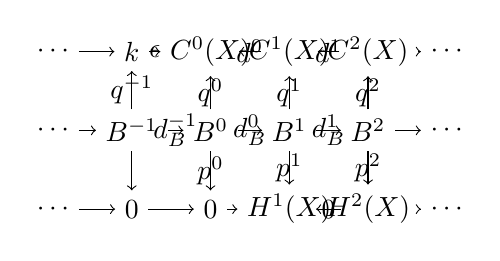
\begin{tikzpicture}
	\node (1) {$k$};
	\node (2) [right of=1] {$C^0(X)$};
	\node (3) [right of=2] {$C^1(X)$};
	\node (4) [right of=3] {$C^2(X)$};
	
	\node (5) [below of=1] {$B^{-1}$};
	\node (6) [right of=5] {$B^0$};
	\node (7) [right of=6] {$B^1$};
	\node (8) [right of=7] {$B^2$};
	
	\node (9) [below of=5] {$0$};
	\node (10) [right of=9] {$0$};
	\node (11) [right of=10] {$H^1(X)$};
	\node (12) [right of=11] {$H^2(X)$};
	
	\node (13) [left of=1] {$\cdots$};
	\node (14) [left of=5] {$\cdots$};
	\node (15) [left of=9] {$\cdots$};
	\node (16) [right of=4] {$\cdots$};
	\node (17) [right of=8] {$\cdots$};
	\node (18) [right of=12] {$\cdots$};
	
	\draw [-to] (13) to node {} (1);
	\draw [-to] (14) to node {} (5);
	\draw [-to] (15) to node {} (9);
	\draw [-to] (4) to node {} (16);
	\draw [-to] (8) to node {} (17);
	\draw [-to] (12) to node {} (18);
	
	\draw [-to] (1) to node {$\epsilon$} (2);
	\draw [-to] (2) to node {$d^0$} (3);
	\draw [-to] (3) to node {$d^1$} (4);
	
	\draw [-to] (5) to node {$d^{-1}_B$} (6);
	\draw [-to] (6) to node {$d^0_B$} (7);
	\draw [-to] (7) to node {$d^1_B$} (8);
	
	\draw [-to] (9) to node {} (10);
	\draw [-to] (10) to node {} (11);
	\draw [-to] (11) to node {$0$} (12);
	
	\draw [-to] (5) to node {$q^{-1}$} (1);
	\draw [-to] (5) to node {} (9);
	
	\draw [-to] (6) to node {$q^0$} (2);
	\draw [-to] (6) to node [swap]{$p^0$} (10);
	
	\draw [-to] (7) to node {$q^1$} (3);
	\draw [-to] (7) to node [swap]{$p^1$} (11);
	
	\draw [-to] (8) to node {$q^2$} (4);
	\draw [-to] (8) to node [swap]{$p^2$} (12);
\end{tikzpicture}
\end{center}

By changing the diagram above slightly at the left-most side, we get the following new diagram:  

\begin{center}
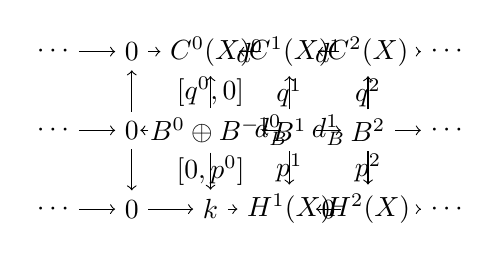
\begin{tikzpicture}
	\node (1) {$0$};
	\node (2) [right of=1] {$C^0(X)$};
	\node (3) [right of=2] {$C^1(X)$};
	\node (4) [right of=3] {$C^2(X)$};
	
	\node (5) [below of=1] {$0$};
	\node (6) [right of=5] {$B^0\oplus B^{-1}$};
	\node (7) [right of=6] {$B^1$};
	\node (8) [right of=7] {$B^2$};
	
	\node (9) [below of=5] {$0$};
	\node (10) [right of=9] {$k$};
	\node (11) [right of=10] {$H^1(X)$};
	\node (12) [right of=11] {$H^2(X)$};
	
	\node (13) [left of=1] {$\cdots$};
	\node (14) [left of=5] {$\cdots$};
	\node (15) [left of=9] {$\cdots$};
	\node (16) [right of=4] {$\cdots$};
	\node (17) [right of=8] {$\cdots$};
	\node (18) [right of=12] {$\cdots$};
	
	\draw [-to] (13) to node {} (1);
	\draw [-to] (14) to node {} (5);
	\draw [-to] (15) to node {} (9);
	\draw [-to] (4) to node {} (16);
	\draw [-to] (8) to node {} (17);
	\draw [-to] (12) to node {} (18);
	
	\draw [-to] (1) to node {} (2);
	\draw [-to] (2) to node {$d^0$} (3);
	\draw [-to] (3) to node {$d^1$} (4);
	
	\draw [-to] (5) to node {} (6);
	\draw [-to] (6) to node {$d^0_B$} (7);
	\draw [-to] (7) to node {$d^1_B$} (8);
	
	\draw [-to] (9) to node {} (10);
	\draw [-to] (10) to node {} (11);
	\draw [-to] (11) to node {$0$} (12);
	
	\draw [-to] (5) to node {} (1);
	\draw [-to] (5) to node {} (9);
	
	\draw [-to] (6) to node {$[q^0, 0]$} (2);
	\draw [-to] (6) to node [swap]{$[0, p^0]$} (10);
	
	\draw [-to] (7) to node {$q^1$} (3);
	\draw [-to] (7) to node [swap]{$p^1$} (11);
	
	\draw [-to] (8) to node {$q^2$} (4);
	\draw [-to] (8) to node [swap]{$p^2$} (12);
\end{tikzpicture}
\end{center}
We see that this in fact gives a span of quasi-isomorphisms $H^*(X)\longleftarrow B'\longrightarrow C^*(X)$, meaning that $X$ is formal. 
\end{proof}

This means that in order to prove that some space is formal, it is enough to prove reduced formality. We can then finally conclude with the following statement.

\begin{corollary}
\label{cor:ls1_then_formal}
Let $X$ be a CW complex with $\ls(X)=1$. Then $X$ is formal.\index{Formal topological space}
\end{corollary}

This result is certainly already known by specialists, but this is seems to be a new method of proving it. It is known because one can show that any space $X$ with $\ls(X)=1$ is a H-cospace, or sometimes called co-H-space (\cite{hess}). Then one can show that a H-cospace is a wedge of copies of $S^1$ and $S_\Q^i$ for some amount of $i$'s, as is done in \cite[Theorem 3.]{co-H-space}. One can also show that formality is preserved under the wedge product (\cite{hess}), and since spheres are formal, we know that any H-cospace, and thus any space $X$ with $\ls(X)\leq 1$ is a formal space. The special case of suspended spaces being formal, was also proven in \cite[Proposition 13.9.]{FHT}. 



\iffalse

\section{Some random applications}

\begin{proposition}
Let $f\colon A\longrightarrow B$ be a morphism between DG-algebras such that both their respective induced product in cohomology is trivial. Then up to a sign we have
\begin{equation*}
    f_*(\langle x_1, x_2, x_3\rangle) = \langle f_*(x_1), f_*(x_2),  f_*(x_3)\rangle.
\end{equation*}
\end{proposition}
\begin{proof}
We get induced $\A$-structures on both $H(A)$ and $H(B)$, and the morphism $f$ induces a morphism $f_*$ in cohomology. We can let $f_*$ be a morphism of $\A$-algebras by letting all of the higher maps be zero. To be precise we have a morphism of $\A$-algebras $g = \{g_n\}$ such that $g_1 = f_*$ and $g_n=0$ for all $n\geq 2$. 

Recall the relation describing the $\A$-morphisms:
\begin{equation*}
    \sum_{n = r+s+t}(-1)^{r+st}g_{r+1+t}(id^{\otimes r}\otimes m_s^A \otimes id^{\otimes t}) = \sum_{k=1}^{n}\sum_{n=i_1+\cdots i_k}(-1)^{u} m_k^B(g_{i_1}\otimes g_{i_2}\otimes \cdots \otimes g_{i_k})
\end{equation*}
where $u=\displaystyle \sum_{t=1}^{k-1}t(i_{k-t}-1)$. Since all the higher maps $g_n$ are zero, the only relations we are left with are the ones only containing $g_1$, i.e. for all $n$ the relation $g_1(m_n^{H(A)}) = m_n^{H(B)}(g_1\otimes \cdots \otimes g_1)$ which is just $f_*(m_n^{H(A)}) = m_n^{H(B)}(f_*\otimes \cdots \otimes f_*)$. For $n=3$ we know that $m_3(x_1, x_2, x_3) = \epsilon \langle x_1, x_2, x_3\rangle$, hence we have (up to a sign)
\begin{equation*}
    f_*(\langle x_1, x_2, x_3\rangle) = \langle f_*(x_1), f_*(x_2),  f_*(x_3)\rangle
\end{equation*}
\end{proof}
\todo[inline]{Maybe add sign?}

Notice that this actually shows a more general statement. If we let $k$ be the smallest number such that $m_k$ is non zero, then the same proof shows that $f_*(\langle x_1, \ldots, x_k\rangle) = \langle f_*(x_1), \ldots, f_*(x_k)\rangle$. 

The above stated result is also just a consequence of the naturality of Massey products we proved earlier in \cref{lm:naturality_of_massey}. There we noted that when the Massey product is uniquely defined, then they are natural on the nose, and not just as a set relation. We still feel that the above result is a nice way to prove it in this special case, as is why we have included it.


\begin{proposition}
Let $A$ be a DG-algebra with trivial induced product on cohomology. For any elements $x_1, x_2, x_3 \in H(A)$ we have
\begin{equation*}
    \langle \langle x_1, x_2, x_3\rangle, x_4, x_5\rangle + (-1)^{|x_1|}\langle x_1,\langle x_2, x_3, x_4\rangle, x_5\rangle + (-1)^{|x_1||x_2|}\langle x_1, x_2, \langle x_3, x_4, x_5\rangle\rangle = 0
\end{equation*}
\end{proposition}
\begin{proof}
Since $m_1 = 0 = m_2$, we have by the fifth Stasheff identity that 
\begin{equation*}
    m_3(m_3\otimes id\otimes id)+m_3(id\otimes m_3\otimes id)+m_3(id\otimes id\otimes m_3)=0 
\end{equation*}
By the Koszul grading convention when applying these operations to elements together with the fact that the Massey products are uniquely defined we get the wanted result. 
\end{proof}

\todo[inline]{Maybe needs an $\epsilon$ in there to get the signs right}

\fi
